% Options for packages loaded elsewhere
\PassOptionsToPackage{unicode}{hyperref}
\PassOptionsToPackage{hyphens}{url}
%
\documentclass[
]{book}
\usepackage{amsmath,amssymb}
\usepackage{lmodern}
\usepackage{iftex}
\ifPDFTeX
  \usepackage[T1]{fontenc}
  \usepackage[utf8]{inputenc}
  \usepackage{textcomp} % provide euro and other symbols
\else % if luatex or xetex
  \usepackage{unicode-math}
  \defaultfontfeatures{Scale=MatchLowercase}
  \defaultfontfeatures[\rmfamily]{Ligatures=TeX,Scale=1}
\fi
% Use upquote if available, for straight quotes in verbatim environments
\IfFileExists{upquote.sty}{\usepackage{upquote}}{}
\IfFileExists{microtype.sty}{% use microtype if available
  \usepackage[]{microtype}
  \UseMicrotypeSet[protrusion]{basicmath} % disable protrusion for tt fonts
}{}
\makeatletter
\@ifundefined{KOMAClassName}{% if non-KOMA class
  \IfFileExists{parskip.sty}{%
    \usepackage{parskip}
  }{% else
    \setlength{\parindent}{0pt}
    \setlength{\parskip}{6pt plus 2pt minus 1pt}}
}{% if KOMA class
  \KOMAoptions{parskip=half}}
\makeatother
\usepackage{xcolor}
\usepackage{longtable,booktabs,array}
\usepackage{calc} % for calculating minipage widths
% Correct order of tables after \paragraph or \subparagraph
\usepackage{etoolbox}
\makeatletter
\patchcmd\longtable{\par}{\if@noskipsec\mbox{}\fi\par}{}{}
\makeatother
% Allow footnotes in longtable head/foot
\IfFileExists{footnotehyper.sty}{\usepackage{footnotehyper}}{\usepackage{footnote}}
\makesavenoteenv{longtable}
\usepackage{graphicx}
\makeatletter
\def\maxwidth{\ifdim\Gin@nat@width>\linewidth\linewidth\else\Gin@nat@width\fi}
\def\maxheight{\ifdim\Gin@nat@height>\textheight\textheight\else\Gin@nat@height\fi}
\makeatother
% Scale images if necessary, so that they will not overflow the page
% margins by default, and it is still possible to overwrite the defaults
% using explicit options in \includegraphics[width, height, ...]{}
\setkeys{Gin}{width=\maxwidth,height=\maxheight,keepaspectratio}
% Set default figure placement to htbp
\makeatletter
\def\fps@figure{htbp}
\makeatother
\setlength{\emergencystretch}{3em} % prevent overfull lines
\providecommand{\tightlist}{%
  \setlength{\itemsep}{0pt}\setlength{\parskip}{0pt}}
\setcounter{secnumdepth}{5}
\usepackage{booktabs}
\usepackage{amsthm}
\makeatletter
\def\thm@space@setup{%
  \thm@preskip=8pt plus 2pt minus 4pt
  \thm@postskip=\thm@preskip
}
\makeatother
\ifLuaTeX
  \usepackage{selnolig}  % disable illegal ligatures
\fi
\usepackage[]{natbib}
\bibliographystyle{apalike}
\IfFileExists{bookmark.sty}{\usepackage{bookmark}}{\usepackage{hyperref}}
\IfFileExists{xurl.sty}{\usepackage{xurl}}{} % add URL line breaks if available
\urlstyle{same} % disable monospaced font for URLs
\hypersetup{
  pdftitle={Lecture Note on Terwilliger Algebra},
  pdfauthor={P. Terwilliger, edited by H. Suzuki},
  hidelinks,
  pdfcreator={LaTeX via pandoc}}

\title{Lecture Note on Terwilliger Algebra}
\author{P. Terwilliger, edited by H. Suzuki}
\date{2022-11-14}

\usepackage{amsthm}
\newtheorem{theorem}{Theorem}[chapter]
\newtheorem{lemma}{Lemma}[chapter]
\newtheorem{corollary}{Corollary}[chapter]
\newtheorem{proposition}{Proposition}[chapter]
\newtheorem{conjecture}{Conjecture}[chapter]
\theoremstyle{definition}
\newtheorem{definition}{Definition}[chapter]
\theoremstyle{definition}
\newtheorem{example}{Example}[chapter]
\theoremstyle{definition}
\newtheorem{exercise}{Exercise}[chapter]
\theoremstyle{definition}
\newtheorem{hypothesis}{Hypothesis}[chapter]
\theoremstyle{remark}
\newtheorem*{remark}{Remark}
\newtheorem*{solution}{Solution}
\begin{document}
\maketitle

{
\setcounter{tocdepth}{1}
\tableofcontents
}
\hypertarget{about-this-lecturenote}{%
\chapter*{About this lecturenote}\label{about-this-lecturenote}}
\addcontentsline{toc}{chapter}{About this lecturenote}

\hypertarget{setting}{%
\section*{Setting}\label{setting}}
\addcontentsline{toc}{section}{Setting}

This note is created by \texttt{bookdown} package on RStudio.

\begin{enumerate}
\def\labelenumi{\arabic{enumi}.}
\tightlist
\item
  Log-in to my GitHub Account
\item
  Go to RStudio/bookdown-demo repository: \url{https://github.com/rstudio/bookdown-demo}
\item
  Use This Template
\item
  Input Repository Name
\item
  Select Public - default
\item
  Create repository from template
\item
  From Code download ZIP
\item
  Move the extracted folder into a favorite directory
\item
  Open RStudio Project in the folder
\item
  Use Terminal in the buttom left pane

  \begin{itemize}
  \tightlist
  \item
    confirm that the current directory is the home directry of the project by pwd
  \end{itemize}
\item
  (failed to proceed by ssh)
\item
  Use Console

  \begin{enumerate}
  \def\labelenumii{\arabic{enumii}.}
  \tightlist
  \item
    library(usethis)
  \item
    use\_git()
  \item
    use\_github() --- Error
  \item
    gh\_token\_help()
  \item
    create\_github\_token(): create a token in the github page. Copy the token
  \item
    gitcreds::gitcreds\_set(): paste the token, the token is to be expired in 30 days
  \end{enumerate}
\item
  Use Terminal

  \begin{enumerate}
  \def\labelenumii{\arabic{enumii}.}
  \tightlist
  \item
    git remote add origin \url{https://github.com/icu-hsuzuki/t-alagebra.git}
  \item
    git push -u origin main
  \item
    type in the password of the computer
  \end{enumerate}
\item
  Use GIT in R Studio
\end{enumerate}

\hypertarget{another-host}{%
\section*{Another Host}\label{another-host}}
\addcontentsline{toc}{section}{Another Host}

\begin{enumerate}
\def\labelenumi{\arabic{enumi}.}
\tightlist
\item
  library(usethis)
\item
  use\_git()
\item
  create\_github\_token()
\item
  gitcreds::gitcreds\_set(): Replace these credentials
\end{enumerate}

\hypertarget{lec1}{%
\chapter{Lecture 1}\label{lec1}}

\textbf{Wednesday, January 20, 1993}

A graph (undirected, without loops or multiple edges) is a pair \(\Gamma = (X, E)\), where
\begin{align}
X &= \textrm{finite set (of vertices)}\\
E & = \textrm{set of (distinct) 2-element subsets of }X \textrm{ (= edges of ) }\Gamma.
\end{align}
vertices \(x\) and \(y\in X\) are adjacent if and only if \(xy\in E\).

\begin{example}

Let \(\Gamma\) be a graph. \(X = \{a, b, c, d\}\), \(E = \{ab, ac, bc, bd\}\).

\begin{center}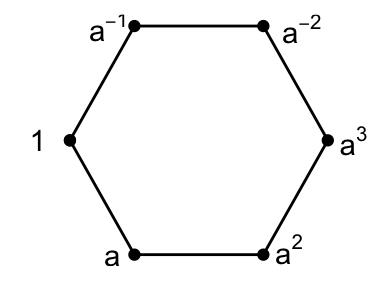
\includegraphics{t-algebra_files/figure-latex/unnamed-chunk-1-1} \end{center}

\end{example}

Set \(n = |X|\), the order of \(\Gamma\).

Pick a field \(K\) (\(=\mathbb{R}\) or \(\mathbb{C}\)). Then \(\mathrm{Mat}_X(K)\) denotes the \(K\) algebra of all \(n\times n\) matrices with entries in \(K\). (rows and columns are indexed by \(X\))

\emph{Adjacency matrix} \(A\in \mathrm{Mat}_X(K)\) is defined by
\begin{align}
A_{xy} & = \left\{\begin{array}{cl} 1 & \textrm{ if } \; xy\in E\\
0 & \textrm{ else } . \end{array}\right.
\end{align}

\begin{example}
Let \(a, b, c, d\) be labels of rows and columns. Then
\[A = \begin{matrix} \\ a\\ b\\c\\d\end{matrix}\begin{matrix}\begin{matrix} a & b & c & d \end{matrix}\\\begin{pmatrix} 0 & 1 & 1 & 0 \\ 1 & 0 & 1 & 1 \\
1 & 1 & 0 & 0 \\ 0 & 1 & 0 & 0 \end{pmatrix}\end{matrix}\]
\end{example}

The subalgebra \(M\) of \(\mathrm{Mat}_X(K)\) generated by \(A\) is called the \emph{Bose-Mesner algebra} of \(\Gamma\).

Set \(V = K^n\), the set of \(n\)-dimensional column vectors, the coorinates are indexed by \(X\).

Let \(\langle\; , \;\rangle\) denote the Hermitean inner product:
\[\langle u, v\rangle = u^\top\cdot v \quad (u, v\in V)\]
\(V\) with \(\langle\; , \;\rangle\) is the \emph{standard module} of \(\Gamma\).

\(M\) acts on \(V\): For every \(x\in X\), write
\[\hat{x} = \begin{pmatrix} 0 \\ \vdots \\ 0 \\ 1 \\ 0 \\ \vdots \\ 0 \end{pmatrix}\]
where \(1\) is at the \(x\) position.

Then
\[A\hat{x} = \sum_{y\in X, xy\in E}\hat{y}.\]
Since \(A\) is a real symmetrix matrix,
\[V = V_0 + V_1 + \cdots + V_r \quad \textrm{ some } r\in \mathbb{Z}^{\geq0},\]
the orthogonal direct sum of maximal \(A\)-eigenspaces.

Let \(E_i\in\mathrm{Mat}_X(K)\) denote the orthogonal projection,
\[E_i: V \longrightarrow V_i.\]
Then \(E_0, \ldots, E_r\) are the primitive idempotents of \(M\).
\[M = \mathrm{Span}_K(E_0, \ldots, E_r),\]
\[E_iE_j = \delta_{ij}E_i \quad \textrm{for all }\; i, j, \quad E_0 + \cdots + E_r = I.\]
Let \(\theta_i\) denote the eigenvalue of \(A\) for \(V_i\) in \(\mathbb{R}\). Without loss of generality we may assume that
\[\theta_0 > \theta_1 > \cdots > \theta_r.\]
Let
\[m_i = \textrm{the multiplicity of }\: \theta_i = \mathrm{dim} V_i = \mathrm{rank} E_i.\]
Set
\[\mathrm{Spec}(\Gamma) = \begin{pmatrix} \theta_0, & \theta_1, & \cdots, & \theta_r\\m_0, & m_1, & \cdots, & m_r\end{pmatrix}.\]
\textbf{Problem. }
What can we say about \(\Gamma\) when \(\mathrm{Spec}(\Gamma)\) is given?

The following Lemma\ref{lem:largestev}, is an example of Problem.

For every \(x\in X\),
\[k(x) \equiv \textrm{ valency of }x \equiv \textrm{ degree of }x \equiv |\{y\mid y\in X, \: xy\in E\}|.\]

\begin{definition}
\protect\hypertarget{def:regular}{}\label{def:regular}The graph \(\Gamma\) is regular of valency \(k\) if \(k = k(x)\) for every \(x\in X\).
\end{definition}

\begin{lemma}
\protect\hypertarget{lem:largestev}{}\label{lem:largestev}With the above notation,\\
1. \(\theta_0\leq \max\{k(x) \mid x\in X\} = k^{\max}\).\\
2. If \(\Gamma\) is regular of valency \(k\), then \(\theta_0 = k\).
\end{lemma}

\begin{proof}

\begin{enumerate}
\def\labelenumi{\arabic{enumi}.}
\tightlist
\item
  Without loss of generality we may assume that \(\theta_0>0\), else done. Let \(v:=\sum_{x\in X}\alpha_x\hat{x}\) denote the eivenvector for \(\theta_0\).
\end{enumerate}

Pick \(x\in X\) with \(|\alpha_x|\) maximal. Then \(|\alpha_x|\neq 0\).

Since \(Av = \theta_0v\),
\[\theta_0\alpha_x = \sum_{y\in X, xy\in E}\alpha_y.\]
So,
\[\theta_0 |\alpha_x| = |\theta_0\alpha_x| \leq \sum_{y\in X, xy\in E}|\alpha_y| \leq k(x)|\alpha_x| \leq k^{\max}|\alpha_x|.\]
2. All 1's vector \(v = \sum_{x\in X}\hat{x}\) satisfies \(Av = kv\).

\end{proof}

\textbf{Subconstituent Algebra}

Let \(x, y\in X\) and \(\ell \in \mathbb{Z}^{\geq 0}\).

\begin{definition}
A path of length \(\ell\) connecting \(x, y\) is a sequence
\[x = x_0, x_1, \ldots, x_{\ell} = y, \quad x_i\in X, \; 0\leq i\leq \ell\]
such that \(x_ix_{i+1}\in E\) for \(0\leq i \leq \ell-1\).
\end{definition}

\begin{definition}
The distance \(\partial(x,y)\) is the length of a shortest path connecting \(x\) and \(y\).
\[\partial(x,y) \in \mathbb{Z}^{\geq 0} \cup \{\infty\}.\]
\end{definition}

\begin{definition}
The graph \(\Gamma\) is connected if and only if \(\partial(x,y) < \infty\) for all \(x, y\in X\).
\end{definition}

From now on, assume that \(\Gamma\) is connected with \(|X|\geq 2\).

Set
\[d_\Gamma = d = \max\{\partial(x,y)\mid x, y\in X\} \equiv \textrm{the diameter of }\Gamma.\]
Fix a `base' vertex \(x\in X\).

\begin{definition}
\[d(x) = \textrm{the diameter with respect to }x = \max\{\partial(x,y)\mid y\in X\} \leq d.\]
\end{definition}

Observe that
\[V = V_0^* + V_1^* + \cdots + V_{d(x)}^* \quad \textrm{(orthogonal direct sum)},\]
where
\[V_i^* = \mathrm{Span}_K(\hat{y}\mid \partial(x,y) = i) \equiv V_i*(x)\]
and \(V_i^* = V_i^*(x)\) is called the \(i\)-the subconstituent with respect to \(x\).

Let \(E_i^* = E_i^*(x)\) denote the orthogonal projection
\[E_i^*: V \longrightarrow V_i^*(x).\]
View \(E_i^*(x) \in \mathrm{Mat}_X(K)\). So, \(E_i^*(x)\) is diagonal with \(yy\) entry
\[(E_i^*(x))_{yy} = \begin{cases} 1 & \textrm{if } \: \partial(x,y) = i\\ 0 & \textrm{else,}\end{cases} \quad \textrm{ for } y\in X.\]
Set
\[M^* = M^*(x) \equiv \textrm{Span}_K(E_0^*(x), \ldots, E_{d(x)}^*(x)).\]
Then \(M^*(x)\) is a commutative subalgebra of \(\mathrm{Mat}_X(K)\) and is calle the \emph{dual Bose-Mesner algbara with respect to \(x\)}.

\begin{definition}[Subconstituent Algebra]
Let \(\Gamma = (X, E)\), \(x\), \(M\), \(M^*(x)\) be as above. Let \(T = T(x)\) denote the subalgebra of \(\mathrm{Mat}_X(K)\) generated by \(M\) and \(M^*(x)\). \(T\) is the \emph{subconstituent algebra} of \(\Gamma\) with respect to \(x\).
\end{definition}

\begin{definition}
A \(T\)-module is any subspace \(W\subset V\) such that \(aw\in W\) for all \(a\in T\) and \(w\in W\).

\(T\)-module \(W\) is \emph{irreducible} if and only if \(W\neq 0\) and \(W\) does not properly contain a nonzero \(T\)-module.
\end{definition}

For any \(a\in \mathrm{Mat}_X(K)\), let \(a^*\) denbote the conjugate transpose of \(a\).

Observe that
\[\langle au, v\rangle = \langle u, a^*v\rangle \quad \textrm{for all }\; a\in \mathrm{Mat}_X(K), \textrm{ and for all } \; u,v\in V.\]

\begin{lemma}

Let \(\Gamma = (X,E)\), \(x\in X\) and \(T \equiv T(x)\) be as above.

\begin{enumerate}
\def\labelenumi{\arabic{enumi}.}
\tightlist
\item
  If \(a\in T\), then \(a^*\in T\).
\item
  For any \(T\)-module \(W\subset V\),
  \[W^\bot := \{v\in V\mid \langle w, v\rangle = 0, \textrm{ for all }w\in W\}\]
  is a \(T\)-module.
\item
  \(V\) decomposes as an orthogonal direct sum of irreducible \(T\)-modules.
\end{enumerate}

\end{lemma}

\begin{proof}

\begin{enumerate}
\def\labelenumi{\arabic{enumi}.}
\item
  It is becase \(T\) is generated by symmetric real matrices
  \[A, E^*_0(x), E^*_1(x), \ldots, E^*_{d(x)(x)}.\]
\item
  Pick \(v\in W^\bot\) and \(a\in T\), it suffices to show that \(av\in W^\bot\). For all \(w\in W\),
  \[\langle w, av\rangle = \langle a^*w, v\rangle = 0\]
  as \(a^*\in T\).
\item
  This is proved by the induction on the dimension of \(T\)-modules. If \(W\) is an irreducible \(T\)-module of \(V\), then
  \[V = W + W^\bot \quad \textrm{(orthogonal direct sum)}.\]
\end{enumerate}

\end{proof}

\textbf{Problem. }
What does the structure of the \(T(x)\)-module tell us about \(\Gamma\)?

Study those \(\Gamma\) whose modules take `simple' form. The \(\Gamma\)'s involved are highly regular.

\begin{remark}

\begin{enumerate}
\def\labelenumi{\arabic{enumi}.}
\tightlist
\item
  The subconstituent algebra \(T\) is semisimple as the left regular representation of \(T\) is completely reducible. See Curtis-Reiner 25.2.
\item
  The inner product \(\langle a, b\rangle_T = \mathrm{tr}(a^\top\bar{b})\) is nondegenerate on \(T\).
\item
  In general,
  \begin{align*}
  T\textrm{: Semisimple and Artinian} & \Leftrightarrow T\textrm{: Artinian with } J(T) = 0 \\
  & \Leftarrow T\textrm{: Artinian with nonzero nilpotent element} \\
  & \Leftarrow T \subset \mathrm{Mat}_X(K) \textrm{ such that for all } a\in T \textrm{ is normal.}
  \end{align*}
\end{enumerate}

\end{remark}

\hypertarget{lec2}{%
\chapter{Lecture 2}\label{lec2}}

\textbf{Friday, January 22, 1993}

In this lecture we use the Perron Frobenius theory of nonnegative matrices to obtain informaiton on eigenvalues of a graph.

Let \(K = \mathbb{R}\). For \(n\in \mathbb{Z}\)\{\textgreater{} 0\}\$, pick a symmetrix matrix \(C\in \mathrm{Mat}_n(\mathbb{R})\).

\begin{definition}
The matrix \(C\) is \emph{reducible} if and only if there is a bipartition \(\{1, 2, \ldots, n\} = X^+ \cup X^-\) (disjoint union of nonempty sets) such that \(C_{ij} = 0\) for all \(i\in X^+\), and for all \(j\in X^-\), and for all \(i\in X^-\), and for all \(j\in X^+\),i.e.,
\[ C \sim \begin{pmatrix} \ast & O \\ O & \ast \end{pmatrix}.\]
\end{definition}

\begin{definition}
The matrix \(C\) is \emph{bipartite} if and only if there is a bipartition \(\{1, 2, \ldots, n\} = X^+ \cup X^-\) (disjoint union of nonempty sets) such that \(C_{ij} = 0\) for all \(i,j\in X^+\), and for all \(i,j\in X^-\), i.e.,
\[ C \sim \begin{pmatrix} O & \ast \\ \ast  & O \end{pmatrix}.\]
\end{definition}

\textbf{Note.}

\begin{enumerate}
\def\labelenumi{\arabic{enumi}.}
\tightlist
\item
  If \(C\) is bipatite, for every eigenvalue \(\theta\) of \(C\), \(-\theta\) is an eigenvalue of \(C\) such that \(\mathrm{mult}(\theta) = \mathrm{mult}(-\theta)\).
\end{enumerate}

Indeed, let \(C = \begin{pmatrix} O & A \\ B & O \end{pmatrix}\),
\[\begin{pmatrix} O & A \\ B & O \end{pmatrix} \begin{pmatrix}x\\y\end{pmatrix} = \theta \begin{pmatrix}x\\y\end{pmatrix}\Leftrightarrow \begin{pmatrix} O & A \\ B & O \end{pmatrix} \begin{pmatrix}x\\-y\end{pmatrix} = -\theta \begin{pmatrix}x\\-y\end{pmatrix}, \]
where \(Ay = \theta x\) and \(Bx = \theta y\).

\begin{enumerate}
\def\labelenumi{\arabic{enumi}.}
\setcounter{enumi}{1}
\item
  If \(C\) is bipartite, \(C^2\) is reducible.
\item
  The matrix \(C\) is irreducible and \(C^2\) is reducible, if \(C_{ij} \geq 0\) for all \(i,j\) and \(C\) is reducible. (Exercise)
\end{enumerate}

\begin{remark}
Note 1. Even if \(C\) is not symmetric
\[\begin{pmatrix} O & A \\ B & O \end{pmatrix} \begin{pmatrix}x\\y\end{pmatrix} = \theta \begin{pmatrix}x\\y\end{pmatrix}\Leftrightarrow \begin{pmatrix} O & A \\ B & O \end{pmatrix} \begin{pmatrix}x\\-y\end{pmatrix} = -\theta \begin{pmatrix}x\\-y\end{pmatrix}\]
holds. So the geometrix multiplicities coincide. How about the algebraic multiplicities?

Note 3. Set \(x \sim y\) if and only if \(C_{xy}>0\). So the graph may have loops. Then
\[(C^2)_{xy} > 0 \Leftrightarrow \textrm{ if there exists } z\in X \textrm{ such that } x\sim z \sim y.\]
Note that \(C\) is irreducible if and only if \(\Gamma(C)\) is connected. Let
\begin{align}
X^+ & = \{y\mid \textrm{there is a path of even length from }x \textrm{ to }y\}\\
X^- & = \{y\mid \textrm{there is no path of even length from }x \textrm{ to }y\} \neq \emptyset.
\end{align}
If there is an edge \(y\sim z\) in \(X^+\) and \(w\in X^-\). Then there would be a path from \(x\) to \(y\) of even length.
So \(\mathrm{e}(X^+, X^+) = \mathrm{e}(X^-, X^-) = 0.\).
\end{remark}

\begin{theorem}[Perron-Frobenius]
\protect\hypertarget{thm:pf}{}\label{thm:pf}

Given a matrix \(C\) in \(\mathrm{Mat}_n(\mathbb{R})\) such that

\begin{enumerate}
\def\labelenumi{\alph{enumi}.}
\tightlist
\item
  \(C\) is symmetric.\\
\item
  \(C\) is irreducible.\\
\item
  \(C_{ij} \geq 0\) for all \(i,j\).
  Let \(\theta_0\) be the maximal eigenvalue of \(C\) with eigenspace \(V_0 \subseteq \mathbb{R}^n\), and let \(\theta_r\) be the maximal eigenvalue of \(C\) with eigenspace \(V_r \subseteq \mathbb{R}^n\). Then the following hold.
\end{enumerate}

\begin{enumerate}
\def\labelenumi{\arabic{enumi}.}
\tightlist
\item
  Suppose \(0\neq v = \begin{pmatrix}\alpha_1\\\alpha_2\\\vdots\\\alpha_n\end{pmatrix} \in V_0\). Then \(\alpha_0 > 0\) for all \(i\), or \(\alpha_i < 0\) for all \(i\).\\
\item
  \(\mathrm{dim}V_0 = 1\).\\
\item
  \(\theta_r \geq -\theta_0\).\\
\item
  \(\theta_r = \theta_0\) if and only if \(C\) is bipartite.
\end{enumerate}

\end{theorem}

First, we prove the following lemma.

\begin{lemma}
\protect\hypertarget{lem:pfl}{}\label{lem:pfl}Let \(\langle , \rangle\) be the dot product in \(V = \mathbb{R}^n\). Pick a symmetric matrix \(B \in \mathrm{Mat}_n(\mathbb{R})\). Suppose all eigenvalues of \(B\) are nonnegative. (i.e., \(B\) is positive semidefinite.) Then there exist vectors \(v_1, v_2, \ldots, v_n\in V\) such that \(B_{ij} = \langle v_i, v_j\rangle\) for \((1\leq i, j \leq n)\).
\end{lemma}

:::\{.proof\}
By elementary linear algebra, there exists an orthonormal basis \(w_1, w_2, \ldots, w_n\) of \(V\) consisting of eigenvectors of \(B\). Set the \(i\)-th column of \(P\) is \(w_i\) and \(D = \mathrm{diag}(\theta_1,\ldots, \theta_n)\). Then \(P^\top P = I\) and \(BP = PD\).

Hence,
\[B = PDP^{-1} = PDP^\top = QQ^\top,\]
where
\[Q = P\cdot \mathrm{diag}(\sqrt{\theta_1}, \sqrt{\theta_2}, \ldots, \sqrt{\theta_n}) \in \mathrm{Mat}_n(\mathbb{R}).\]
Now, let \(v_i\) be the \(i\)-th column of \(Q^\top\). Then
\[B_{ij} = v_i^\top\cdot v_j^- = \langle v_i, v_j\rangle.\]
Now we start the proof of Theorem \ref{thm:pf}.

\emph{Proof of Theorem \ref{thm:pf}}

\begin{enumerate}
\def\labelenumi{\arabic{enumi}.}
\tightlist
\item
  Let \(\langle , \rangle\) denote the dot product on \(V = \mathbb{R}^n\). Set
  \begin{align}
  B & = \theta I - C\\
    & = \textrm{symmetric matrix with eigenvalues }\theta_0 - \theta_i \geq 0\\
    & = (\langle v_i, v_j\rangle)_{1\leq i,j\leq n}
  \end{align}
  with the same \(v_1, \ldots, v_n \in V\) by Lemma \ref{lem:pfl}.
\end{enumerate}

Observe: \(\sum_{i = 1}^n \alpha_iv_i = 0\).

\emph{Pf.}
\begin{align}
\|\sum_{i = 1}^n \alpha_iv_i\|^2 & = \langle \sum_{i=1}^n\alpha_iv_i, \sum_{i=1}^n\alpha_iv_i\rangle\\
& = \begin{pmatrix} \alpha_1 &\ldots &\alpha_n\end{pmatrix}B\begin{pmatrix} \alpha_1\\\vdots\\\alpha_n\end{pmatrix}\\
& = v^\top Bv\\
& = 0,
\end{align}
since \(Bv = (\theta_0 I - C)v = 0\).

Now set
\[s = \textrm{the number of indices} i, \textrm{ where } \alpha_i >0.\]
Replacing \(v\) by \(-v\) if necessary, without loss of generality we may assume that \(s\geq 1\). We want to show \(s = n\).

Assume \(s < n\). Without loss of generality, we may assume that \(\alpha_i >0\) for \(1\leq s\leq s\) and \(\alpha_i = 0\) for \(s+1 \leq i \leq n\).
Set
\[ \rho = \alpha_1v_1 + \cdots + \alpha_sv_s = -\alpha_{s+1}v_{s+1} - \cdots - \alpha_nv_n.\]
Then, for \(i = 1,\ldots, s\),
\begin{align}
\langle v_i, \rho \rangle & = \sum_{j = s+1}^n -\alpha_j\langle v_i, v_j\rangle \quad (\langle v_i, v_j\rangle = B_{ij}, B = \theta_0I - C)\\
  & = \sum_{j = s+1}^n (-\alpha_{ij})(-C_{ij})\\
  & \leq 0.
\end{align}
Hence
\[0\leq \langle \rho, \rho\rangle = \sum_{i=1}^s \alpha_i \langle v_i, \rho\rangle \leq 0,\]
as \(\alpha > 0\) and \(\langle v_i, \rho\rangle \leq 0\). Thus, we have
\(\langle, \rho, \rho \rangle = 0\) and \(\rho = 0\).
For \(j = s+1, \ldots, n\),
\[0 = \langle \rho, v_j\rangle = \sum_{i=1}^s \alpha_i\langle v_i, v_j\rangle \leq 0,\]
as \(\langle v_i, v_j\rangle = -C_{ij}\).

Therefore,
\[0 = \langle v_i, v_j \rangle = -C_{ij} \textrm{ for } 1\leq i, \leq s, \: s+1 \leq j \leq n.\]
Since \(C\) is symmetric,
\[C = \begin{pmatrix} \ast & O \\ O & \ast\end{pmatrix}\]
Thus \(C\) is reducible, which is not the case. Hence \(s = n\).

\emph{Proof of Theorem \ref{thm:pf} 2.}

Suppose \(\dim V_0 \geq 2\). Then,
\[\dim\left(V_0 \cap \begin{pmatrix}1\\0\\\vdots\\0\end{pmatrix}^\bot\right) \geq 1.\]
So, there is a vector
\[0\neq v = \begin{pmatrix}\alpha_1\\\vdots\\\alpha_n\end{pmatrix} \in V_0\]
with \(\alpha_1 = 0\). This contradicts 1.

Now pick
\[0\neq w = \begin{pmatrix}\beta_1\\\vdots\\\beta_n\end{pmatrix} \in V_r.\]

\emph{Proof of Theorem \ref{thm:pf} 3.}

Suppose \(\theta_r < -\theta_0\). Since the eigenvalues of \(C^2\) are the squares of those of \(C\), \(\theta_r^2\) is the maximal eigenvalue of \(C^2\).

Also we have \(C^2w = \theta_r^2w\).

Observe that \(C^2\) is irreducible. (As otherwise, \(C\) is bipartite by Note 3, and we must have \(\theta_r = -\theta_0\).)
Therefore, \(\beta_i > 0\) for all \(i\) or \(\beta_i < 0\) for all \(i\). We have
\[\langle v, w\rangle = \sum_{i=1}^n\alpha_i\beta_j \neq 0.\]
This is a contradiction, as \(V_0 \bot V_r\).

\emph{Proof of Theorem \ref{thm:pf} 4.}

\(\Rightarrow\): Let \(\theta_r = -\theta_0\). Then \(\theta = \theta_1^2 = \theta_0^2\) is the maximal eigenvalue of \(C^2\), and \(v\) and \(w\) are linearly independent eigenvalues for \(\theta\) for \(C^2\). Hence, for \(C^2\), \(\mathrm{mult}(\theta) \geq 2\).

Thus by 2, \(C^2\) must be reducible. Therefore, \(C\) is bipartite by Note 3.

\(\Leftarrow\): This is Note 1.
\(\Box\)

Let \(\Gamma = (X, E)\) be any graph.

\begin{definition}
\(\Gamma\) is said to be \emph{bipartite} if the adjacency matrix \(A\) is bipartite. That is, \(X\) can be written as a disjoint union of \(X^+\) and \(X^-\) such that \(X^+, X^-\) contain no edges of \(\Gamma\).
\end{definition}

\begin{corollary}

For any (connected) graph \(\Gamma\) with
\[\mathrm{Spec}(\Gamma) = \begin{pmatrix}\theta_0 & \theta_1 &\cdots & \theta_r\\m_1 & m_1 & \cdots & m_r\end{pmatrix} \:\textrm{ with }\: \theta_0 > \theta_1 > \cdots > \theta_r.\]
Let \(V_i\) be the eigenspace of \(\theta_i\). Then the following holds.

\begin{enumerate}
\def\labelenumi{\arabic{enumi}.}
\item
  Supppose \(0\neq v = \begin{pmatrix} \alpha_1\\\vdots \\\alpha_n \end{pmatrix} \in V_0\in \mathbb{R}^n\). Then \(\alpha_i > 0\) for all \(i\) or \(\alpha_i < 0\) for all \(i\).
\item
  \(m_0 = 1\).
\item
  \(\theta_r \geq -\theta_0\) if and only if \(\Gamma\) is bipartite. In this case,
  \[-\theta_i = \theta_{r-i} \; \textrm{and} \; m_i = m_{r-i} \quad (0\leq i\leq r)\]
\end{enumerate}

\end{corollary}

\begin{proof}
This is a direct consequences of Theorem \ref{thm:pf} and Note 3.
\end{proof}

\hypertarget{lec3}{%
\chapter{Lecture 3}\label{lec3}}

\textbf{Monday, January 25, 1993}

Given graphs \(\Gamma = (X, E)\) and \(\Gamma' = (X', E')\).

\begin{example}

\(\Delta = \{a, a^{-1}\}\)

\begin{center}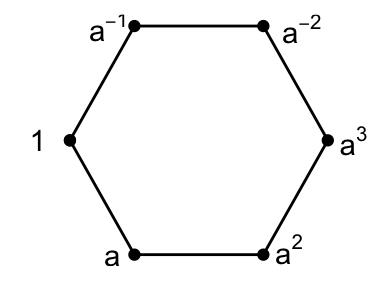
\includegraphics{t-algebra_files/figure-latex/unnamed-chunk-2-1} \end{center}

\end{example}

\begin{example}

\(\Delta = \{a, a^{-1}, a^2, a^{-2}\}\)

\begin{center}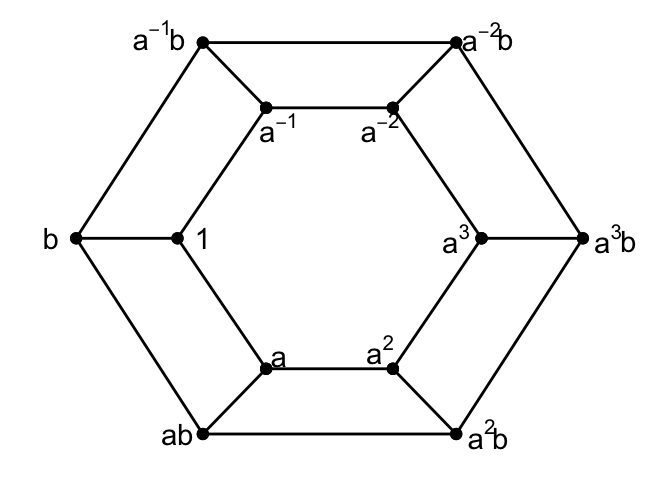
\includegraphics{t-algebra_files/figure-latex/unnamed-chunk-3-1} \end{center}

\end{example}

\begin{example}

\(G = \langle a, b \mid a^6 = 1, b^2, ab = ba\rangle\), \(\Delta = \{a, a^{-1}, b\}\)

\begin{center}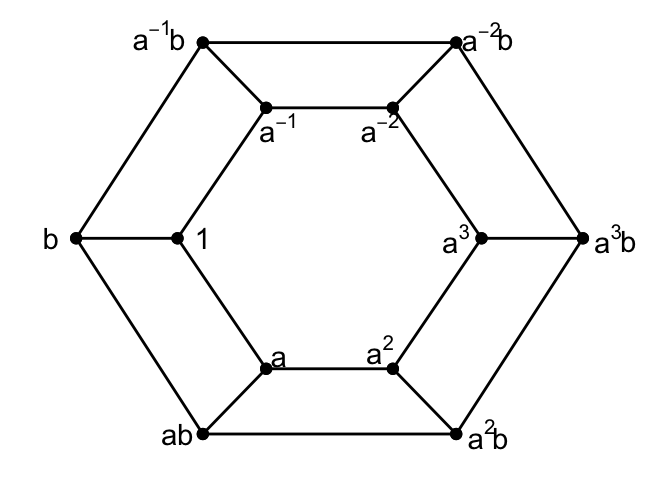
\includegraphics{t-algebra_files/figure-latex/unnamed-chunk-4-1} \end{center}

\end{example}

\hypertarget{applications}{%
\chapter{Applications}\label{applications}}

Some \emph{significant} applications are demonstrated in this chapter.

\hypertarget{example-one}{%
\section{Example one}\label{example-one}}

\hypertarget{example-two}{%
\section{Example two}\label{example-two}}

\hypertarget{final-words}{%
\chapter{Final Words}\label{final-words}}

We have finished a nice book.

  \bibliography{book.bib,packages.bib}

\end{document}
